\chapter{Rekurzívne clustrovanie pod dohľadom užívateľa}

Všetky algoritmy zmienené v predchádzajúcej kapitole pomerne dobre odhaľujú parsovacie vzory, ktoré sa v danom datasete objavujú často a výsledky sú presné. Ale aby sme dosiahli odhalenie všetkých parsovacích vzorov, pri zachovaní vysokej presnosti, musíme sa vysporiadať s obmedzeniami clustrovacích algoritmov \parencite{Tovarnak2017}.

\subsection*{Rozdelenie správy na token}
Prvým krokom všetkých prezentovaných algoritmom je rozdeliť parsovaciu správu na tokeny. V tomto smere je potrebná väčšia variabilita pri zadávaní oddeľovača slov. Nie všetky algoritmy podporujú možnosť zadať aj iný oddeľovač ako medzera, ale ani podpora pre viac oddeľovačov tokenov nie je dostačujúca ako si ukážeme na príklade. \\

\indent \emph{Starting server with param timeout=2000 ms} \\
\indent \emph{Processing request 127.0.0.1/api/patterns?page-size=10\&page=3} \\

V prvom prípade chceme použiť ako delimiter aj znak \emph{=} . V druhom prípade je žiaduce, aby celá url bola zachytená ako jeden parameter. Delimiter \emph{=} teda použiť nechceme. Preto možnosť použiť iný delimiter pre rôzne logovacie správy by pomohla ďalej spresniť výsledné parsovacie vzory.

\subsection*{Vstupné parametre}
Hodnota vstupných parametrov je vo vačšine prípadov jedným z hlavných faktorov, ktorý ovplyvňuje kvalitu výsledných parsovacích vzorov.
Pre tieto hodnoty existujú odporúčania, ale najpresnejší výsledok získame až po manuálnej analýze datasetu, kde užívateľ po prezretí správ datasetu spustí pár krát daný algoritmus a pokúsi sa nájsť parametre, pre ktoré budú výsledné parsovacie vzory čo najpresnejšie.

\subsection*{Kontrola výsledných parsovacích vzorov}
V závislosti od vyššie zmienených nastavení dostaneme parsovacie vzory, ktoré buď zodpovedajú našej predstave alebo nie. Komplikovanejšia situácia nasáva v prípade, ak neexistuje všeobecné nastavenie algoritmu, ktoré by vrátilo všetky parsovacie vzory v potrebnej kvalite. Tento problém sa dá obísť užívateľským rozdelením datasetu na menšie časti a na každú časť pustiť algoritmus s vlastným nastavením. Toto je ale komplikované, zdĺhavé, náchylne k chybám a v neposlednom rade aj užívateľsky neprívetivé.

\section{RURC - Recursive User-Reviewed Clustering}
Z hore uvedeného rozboru vyplýva, že ideálny algoritmus by mal zahrňovať určitý stupeň užívateľskej interakcie a mal by vedieť pracovať aj nad vybranou podmnožinou daného datasetu. Vedúci práce preto v \parencite{Tovarnak2017} navrhol systematický postup nazvaný \emph{Recursive User-Reviewed Clustering} znázornený na obr. \ref{fig:rurc}. Výsledkom je proces, pri ktorom užívateľ rekurzívne spúšťa algoritmus nad datasetom, pričom v každom priebehu má možnosť potvrdiť finálne parsovacie vzory a odfiltrovať z datasetu správy ktoré k nim patria. Tento proces prebieha v týchto krokoch:

\begin{enumerate}
  \item Odstránenie správ z datasetu, ktoré prislúchajú k už odhaleným parsovacím vzorom.
  \item Úvodný beh algoritmu s defaultnými parametrami.
  \item Užívateľ rozhodne, ktoré parsovacie vzory sú akceptovateľné, tým zároveň z datasetu odstráni príslušné správy.
  \item Užívateľ buď:
  	\begin{enumerate}
   		 \item Spustí algoritmus nad celým datasetom so zmenenými parametrami. A pokračuje od bodu 3.
   		 \item Označí množinu vzorov, ktoré nie sú vhodné a spustí algoritmus nad podmnožinou datasetu, ktorá prísluší k vybraným vzorom a 				pokračuje od bodu 3.
   		 \item Ukončí proces. Proces tiež končí, ak už neostali žiadne správy na spracovanie.
 	 \end{enumerate}
\end{enumerate}

\begin{figure}[htbp]
 \centering 
 \begin{minipage}{0.95\linewidth}
 	\centering
 	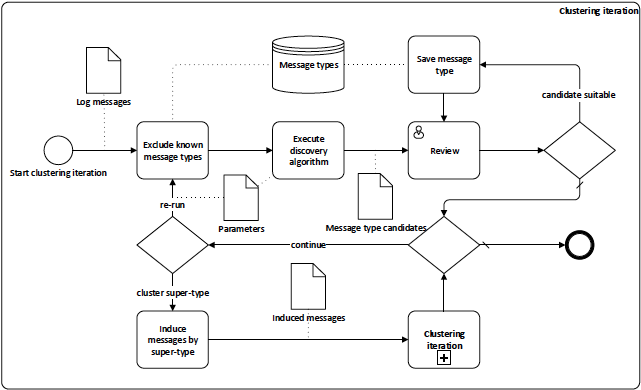
\includegraphics[width=\textwidth]{images/RURC.png} 	
 \end{minipage}
  \caption{Recursive User-Reviewed Clustering, obr. prevzaný z  \parencite{Tovarnak2017}}
  \label{fig:rurc}
\end{figure}


\section{Extended Nagappan-Vouk algoritmus}
RURC definuje obecné princípy analýzy logovacích súborov, nešpecifikuje algoritmus, ktorý má byť použitý na clustrovanie správ.
Z nedostatkov zmienených v predchádzajúcej kapitole ale vyplýva, že žiaden algoritmus okrem LogCluster sa nehodí na použitie v RURC.
Vedúci práce preto vyvinul algoritmus Extended Nagappan-Vouk, určený pre použitie v RURC, ktorý bude spĺnať všetky požiadavky RURC a zároveň bude jednoduchšie nastaviteľný ako LogCluster. Algoritmus produkuje parsovacie vzory vo formáte $\%\{m,n\}$, ktorý podobne ako pri LogClustry znamená \emph{m} až \emph{n} za sebou idúcich tokenov. Postup algoritmu: 

\begin{enumerate}
 \item V prvom kroku sa správy rozdelia na tokeny na základe užívateľom zadaných oddeľovačou slov.
 \item V druhom kroku algoritmus vybuduje frekvenčnú tabuľku rovnako ako pri klasickom Nagappan-Vouk. Rozdiel je, že algoritmus si ukladá aj pozície rozdeľovačov slov.
 \item Pre každú správu si vo frekvenčnej tabuľke vyhľadáme frekvencie všetkých tokenov správy. Rozdiel oproti Nagappan-Vouk je ten, že hraničnú frekvenciu určíme metódou q-percentilu poďla užívateľom zadanej vstupnej hodnoty. Podľa toho označím tokeny ako statickú časť alebo wildcard.
 \item Použitím heuristiky algoritmus skúsi odhaliť prekrývajúce sa clustre a v prípade, že také clustre existujú pripojí špecifickejší cluster k viac všeobecnému.
 \item Algoritmus detekuje po sebe idúce sekvencie wildcard v doposiaľ nájdených vzoroch a ak je to možné tieto sekvencie spojí a vytvorí
 vzor s dolnou a hornou hranicou spojených tokenov.
\end{enumerate}



